\documentclass[a4paper,12pt]{article}
\usepackage{graphicx}
\usepackage{verbatim}
\usepackage{amsmath}
\begin{document}
	\title{\textbf{Homework1 Rostagno}}
	\author{295706}
	\date{\today}
	\maketitle
	
	\centering \textbf{Esercizio 1}\\
	\begin{itemize}
		\item \textbf{Punto a: } 
		\begin{align*}
			U &= \{o\} & U^c &= \{a, b, c, d\} & C_U &= 6 \\
			U &= \{o, a\} & U^c &= \{b, c, d\} & C_U &= 6 \\
			U &= \{o, b\} & U^c &= \{a, c, d\} & C_U &= 8 \\
			U &= \{o, c\} & U^c &= \{a, b, d\} & C_U &= 7 \\
			U &= \{o, a, b\} & U^c &= \{c, d\} & C_U &= 7 \\
			U &= \{o, b, c\} & U^c &= \{a, d\} & C_U &= 6 \\
			U &= \{o, a, c\} & U^c &= \{b, d\} & C_U &= 7 \\
			U &= \{o, a, b, c\} & U^c &= \{d\} & C_U &= 5 \\
			\end{align*}
			Ho calcolato la capacità di ogni taglio ($C_U$) dividendo insieme di partenza (U) e insieme di arrivo ($U^c$). \\
			La capacità minima da rimuovere affinché non sia più possibile alcun flusso fattibile dal nodo $o$ al nodo $d$ è 5, va rimossa dagli archi $e_2$ $e_4$ $e_6$.
			\item \textbf{Punto b: } Sia $x$ la capacità extra da aggiungere, per poter massimizzare il throughput da o a d è necessario aggiungere la capacità su degli archi prestabiliti in un certo ordine. Dobbiamo inserire la prima unità sull'arco $e_2$, successivamente va aggiunta su $e_4$, poi su $e_1$ ed infine su $e_3$; dopodichè si ricomincia da $e_2$ e si ripete in base al valore di $x$. Questa è la sequenza che aumenta in maniera più rapida il throughput.\\
			Graficamente diventa:
			\begin{figure}[h] % L'ambiente figure permette di gestire il posizionamento
				\centering % Centra l'immagine
				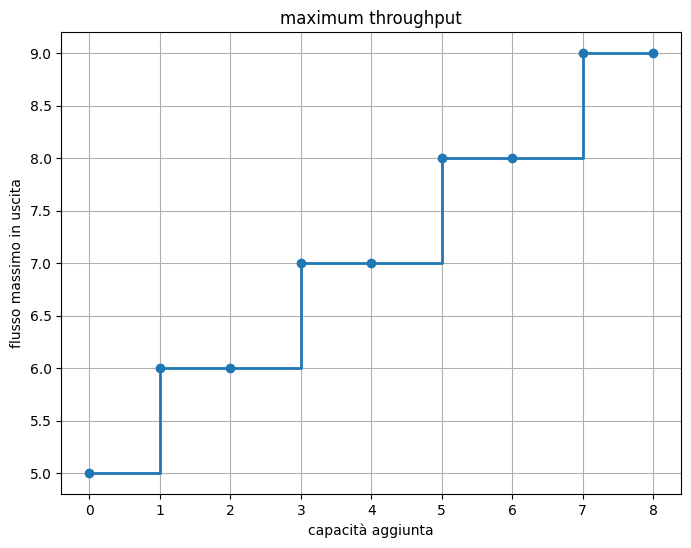
\includegraphics[width=0.8\textwidth]{graf1.png} % Inserisce l'immagine con larghezza metà pagina
				\caption{Massimo flusso in uscita in base alla capacità aggiunta} % Aggiunge una didascalia all'immagine
				\label{fig:immagine} % Aggiunge un'etichetta per riferimenti interni
			\end{figure}
			\newpage
			Nel caso in cui non si aggiunga capacità extra abbiamo come flusso max 5, se aggiungiamo una o due unità di capacità otteniamo 6 come flusso max mentre se aggiungiamo tre o quattro unità di capacità otteniamo 7 come flusso max. Dopo questi 4 valori notiamo che il grafico si ripete (come detto in precedenza).
			\item \textbf{Punto c: }Il nuovo collegamento $e_8$ di capacità 1 dovrebbe essere aggiunto in una posizione che contribuisca a migliorare il taglio minimo, di conseguenza l'ho aggiunto tra il nodo $c$ e il nodo $d$ in quanto era il collegamento più debole. La posizione delle capacità segue un andamento periodico come prima, vanno inserite in questo ordine e poi ripetute: $e_3, e_2, e_4, e_1$.
			Graficamente diventa:
			\begin{figure}[h] % L'ambiente figure permette di gestire il posizionamento
				\centering % Centra l'immagine
				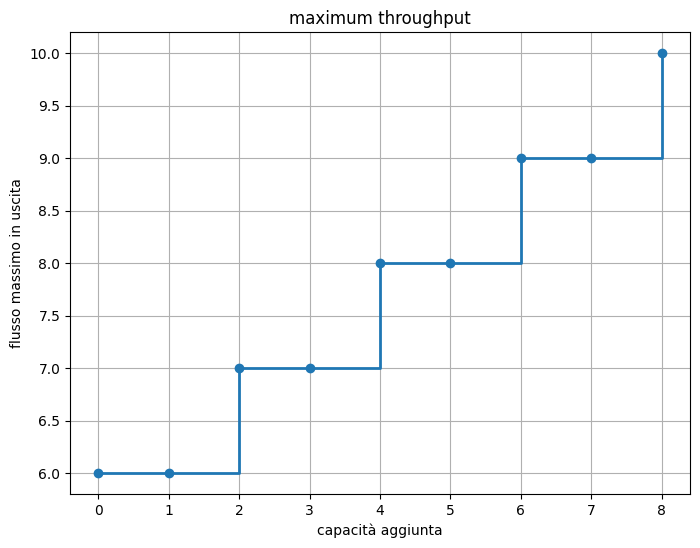
\includegraphics[width=0.8\textwidth]{graf2.png} % Inserisce l'immagine con larghezza metà pagina
				\caption{Massimo flusso in uscita in base alla capacità aggiunta} % Aggiunge una didascalia all'immagine
				\label{fig:immagine} % Aggiunge un'etichetta per riferimenti interni
			\end{figure}
			\newpage
			Notiamo che la capacità iniziale è aumentata di 1 e che dopo ogni 4 unità aggiunte il grafico si ripete.
	\end{itemize}
		\centering \textbf{Esercizio 2}\\
		\begin{itemize}
			\item \textbf{Punto a: }Considerando che il throughput è uguale a 2 e si inserisce nel vertice $o$, abbiamo tre possibili percorsi che il flusso può seguire:
			\begin{itemize}
				\item Percorso 1: $e_5, e_6$
				\item Percorso 2: $e_1, e_2, e_4$
				\item Percorso 3: $e_1, e_3, e_4$
			\end{itemize}
			Chiamiamo le nostre quattro variabili di flusso $x_1x_2x_3x_4$ dove $x_1$ rappresenta il flusso in $e_1$, $x_2$ rappresenta il flusso in $e_5$, $x_3$ rappresenta il flusso in $e_3$ e $x_4$ rappresenta il flusso in $e_2$. Ora scriviamo il nostro problema di ottimizzazione:\\
			\[
			\begin{aligned}
				&\min_{x_1, x_2, x_3, x_4} \quad f(x) = x_2 \cdot (2 x_2 + 2 + 3 x_2) + x_1 \cdot (3 x_1 + x_1 + 1) + 3 x_3 + x_4 \cdot (x_4 + 1) \\
				&\text{vincoli:} \\
				&x_1 + x_2 = 2, \\
				&x_3 + x_4 = x_1, \\
				&x_1,x_2,x_3,x_4 \geq 0.
			\end{aligned}
			\]
			Facendo le opportune sostituzioni e gli opportuni calcoli si ottiene che la funzione viene minimizzata con $x=[1,1,0,1]$. Notiamo quindi che l'arco $e_3$ non viene utilizzato e che il flusso iniziale si divide a metà (un'unità nel percorso 2 ed un'unità nel percorso 1).\\
			Costo totale=14.
			\item \textbf{Punto b: } Sicuramente non esiste un flusso che permetta di avere il costo del pedaggio dei 3 percorsi uguale, in quanto il percorso 2 e il percorso 3 hanno due archi in comune e uguagliare gli archi $e_2,e_3$ vorrebbe dire avere un flusso di 2 unità nell'arco $e_2$, ma questo non è possibile perchè vorrebbe dire avere un pedaggio nullo nel percorso 1. Possiamo quindi eguagliare il costo del pedaggio del percorso 1 al percorso 2 o al percorso 3. Nel primo caso otteniamo lo stesso flusso del punto a, ovvero $x_1=1$ e $x_2=1$. Nel secondo caso invece otteniamo $x_1=\frac{8}{9}$ e $x_2=\frac{10}{9}$.\\
			I costi totali sono rispettivamente 14 per i percorsi 1 e 2, e $\frac{136}{9}$ per i percorsi 1 e 3.\\
			I prezzi di anarchia sono corrispettivamente 1 e $\frac{68}{63}$.
			\end{itemize}
\end{document}